\subsection{APDU Packets}\label{subsec:apdu}
\ch{fix crefs to tables}
Communication between a smart card and a terminal is done via packets called Application Protocol Data Units (APDU). There are two types of communication packets: command and response. The structure of the packets can be seen in \cref{tab:apduCommand} and \cref{tab:apduResponse}, respectively.\\\\
The command APDU has four mandatory header bytes (CLA, INS, P1, P2), some optional command data. $L_{c}$ encodes the length of the command data, and $L_{e}$ encodes the maximum number of bytes expected in the response APDU.\\\\
The response apdu has optional response data followed by two mandatory status bytes (SW1, SW2) indicating the status of the command request sent to the card.

\begin{table}[H]
	\centering
    \begin{tabular}{|l|l|l|l|l|l|}
    \hline
    CLA & INS & P1 - P2 & $L_{c}$ & Command Data & $L_{e}$ \\ \hline
    \end{tabular}
    \caption{The structure of a command APDU}
    \label{tab:apduCommand}
\end{table}

\begin{table}[H]
	\centering
    \begin{tabular}{|l|l|}
    \hline
    Response Data & SW1 - SW2 \\ \hline
    \end{tabular}
    \caption{The structure of a response APDU}
    \label{tab:apduResponse}
\end{table}

Communication is always initated by the terminal by sending a command APDU - the \jc may or may not reply to the command with a response APDU. \cref{fig:apdu} illustrates that a command APDU packet is sent from a terminal to a smart card. The command packet is then processed and a response might be sent from the smart card to the terminal.
 
\begin{figure}[H]
  \centering
  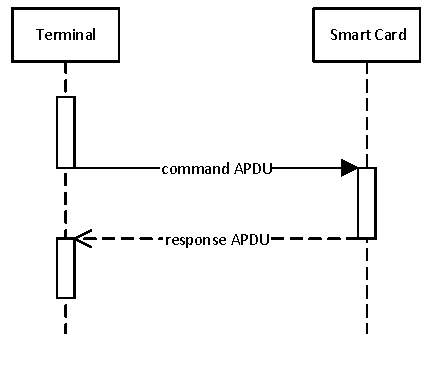
\includegraphics[scale=1, trim=0cm 0cm 0cm 0cm]{figures/apdu}
  \caption{Communication between a terminal and a \jc via command and response APDUs. Figure from~\cite[p. 4]{javasec}.}
  \label{fig:apdu}
\end{figure}